\documentclass[twoside, a4paper, 12pt]{book}



%:-------------------------- packages for fancy things -----------------------

\usepackage{amssymb, amsmath}
\usepackage{graphics} % for improved inclusion of graphics
%\usepackage{wrapfig} % to include figure with text wrapping around it
\usepackage[margin=10pt,font=small,labelfont=bf]{caption} % for improved layout of figure captions with extra margin, smaller font than text
\usepackage{fancyhdr} % for better header layout
\usepackage{eucal}
\usepackage[english]{babel}
\usepackage[usenames, dvipsnames]{color}
\usepackage[perpage]{footmisc}
%\usepackage[round, sort, numbers, authoryear]{natbib}
\usepackage{ifthen}
\usepackage{multicol} % for pages with multiple text columns, e.g. References
\setlength{\columnsep}{20pt} % space between columns; default 10pt quite narrow
\usepackage[nottoc]{tocbibind} % correct page numbers for bib in TOC, nottoc suppresses an entry for TOC itself
%\usepackage{nextpage}

\usepackage{lmodern}

\usepackage{algorithmic}
\usepackage{algorithm}
%\usepackage{program}

\numberwithin{algorithm}{chapter}

\usepackage[utf8x]{inputenc}

%:-------------------------- Glossary/Abbrev./Symbols -----------------------

\usepackage[intoc]{nomencl} % load nomencl extension; include in TOC
%\nomrefpage % to include page numbers after abbrevations
\renewcommand{\nomname}{Glossary} % rename nomenclature
\renewcommand{\nomlabel}[1]{\textbf{#1}} % make abbreviations bold
\makenomenclature % used to be \makeglossary
\newcommand{\g}{\footnote{For all abbreviations see the glossary on page \pageref{nom}.}} % type "\g" to refer to glossary




% used to be for sorting into categories:
%\renewcommand\nomgroup[1]{%
%  \ifthenelse{\equal{#1}{A}}{%
%   \item[\textbf{Roman Symbols}] }{%             A - Roman
%    \ifthenelse{\equal{#1}{G}}{%
%     \item[\textbf{Greek Symbols}]}{%             G - Greek
%      \ifthenelse{\equal{#1}{R}}{%
%        \item[\textbf{Superscripts}]}{%              R - Superscripts
%          \ifthenelse{\equal{#1}{S}}{%
%           \item[\textbf{Subscripts}]}{{%             S - Subscripts
%	    \ifthenelse{\equal{#1}{X}}{%
%	     \item[\textbf{Other Symbols}]}{{%    X - Other Symbols
%	    \ifthenelse{\equal{#1}{Z}}{%
%	     \item[\textbf{Acronyms}]}%              Z - Acronyms
%              			{{}}}}}}}}}}



%-------Hyperref and graphics ---------------%
\usepackage[ pdftex, plainpages = false, pdfpagelabels, 
                 pdfpagelayout = useoutlines,
                 bookmarks,
                 bookmarksopen = true,
                 bookmarksnumbered = true,
                 breaklinks = true,
                 linktocpage,
                 pagebackref,
                 colorlinks = false,  % was true
                 linkcolor = blue,
                 urlcolor  = blue,
                 citecolor = red,
                 anchorcolor = green,
                 hyperindex = true,
                 hyperfigures
                 ]{hyperref} 

\DeclareGraphicsExtensions{.png, .jpg, .jpeg, .pdf, .gif} %GIF doesn't work??
\usepackage[pdftex]{graphicx}
\pdfcompresslevel=9
%\graphicspath{{0_frontmatter/figures/PNG/}{0_frontmatter/figures/PDF/}{0_frontmatter/figures/}}


%:-------------------------- page layout -----------------------

%A4 settings

\pdfpageheight=297mm
\pdfpagewidth=210mm


\setlength{\hoffset}{0.00cm}
\setlength{\voffset}{0.00cm}

%: Uncomment this secion for two-sided printing
% ------------------------------
\setlength{\oddsidemargin}{1.5cm}
\setlength{\evensidemargin}{0cm}
\setlength{\topmargin}{1mm}
\setlength{\headheight}{1.36cm}
\setlength{\headsep}{1.00cm}
\setlength{\textheight}{20.84cm}
\setlength{\textwidth}{14.5cm}
\setlength{\marginparsep}{1mm}
\setlength{\marginparwidth}{3cm}
\setlength{\footskip}{2.36cm}


%: Uncomment this secion for one-sided printing
% taken from the original file, but with the first two lanes modified
% ------------------------------
%\setlength{\evensidemargin}{1.9cm} % was 1.96cm in original
%\setlength{\oddsidemargin}{-0.001cm} % was -0.54cm in original file
%\setlength{\topmargin}{1mm}
%\setlength{\headheight}{1.36cm}
%\setlength{\headsep}{1.00cm}
%\setlength{\textheight}{20.84cm}
%\setlength{\textwidth}{14.5cm}
%\setlength{\marginparsep}{1mm}
%\setlength{\marginparwidth}{3cm}
%\setlength{\footskip}{2.36cm}


%: section below defines fancy page layout options
% ------------------------------
\pagestyle{fancy}
\renewcommand{\chaptermark}[1]{\markboth{\MakeUppercase{\thechapter. #1 }}{}}
\renewcommand{\sectionmark}[1]{\markright{\thesection\ #1}}
\fancyhf{}
\fancyhead[RO]{\bfseries\rightmark}
\fancyhead[LE]{\bfseries\leftmark}
\fancyfoot[C]{\thepage}
\renewcommand{\headrulewidth}{0.5pt}
\renewcommand{\footrulewidth}{0pt}
\addtolength{\headheight}{0.5pt}
\fancypagestyle{plain}{
  \fancyhead{}
  \renewcommand{\headrulewidth}{0pt}
}





%:-------------------------- title page layout -----------------------

% starts roman page numbering until chapter 1
% important to avoid two pages numbered 1 and 2 which may cause bad links
% bug: cover i + back side ii and then numbering restarts with i; should be iii
\renewcommand{\thepage}{\roman{page}}

\newcommand{\submittedtext}{{A thesis submitted for the degree of}}

% DECLARATIONS
% These macros are used to declare arguments needed for the
% construction of the title page and other preamble.

% The year and term the degree will be officially conferred
\def\degreedate#1{\gdef\@degreedate{#1}}
% The full (unabbreviated) name of the degree
\def\degree#1{\gdef\@degree{#1}}
% The name of your college or department(eg. Trinity, Pembroke, Maths, Physics)
\def\collegeordept#1{\gdef\@collegeordept{#1}}
% The name of your University
\def\university#1{\gdef\@university{#1}}
% Defining the crest
\def\crest#1{\gdef\@crest{#1}}
% Stating the city of birth for title page where needed; uncommented for use
%\def\cityofbirth#1{\gdef\@cityofbirth{#1}}

% These macros define an environment for front matter that is always 
% single column even in a double-column document.
\newenvironment{alwayssingle}{%
       \@restonecolfalse\if@twocolumn\@restonecoltrue\onecolumn
       \else\newpage\fi}
       {\if@restonecol\twocolumn\else\newpage\fi}

%:-------------------------- front matter layout -----------------------

% DEDICATION
%
% The dedication environment makes sure the dedication gets its
% own page and is set out in verse format.

\newenvironment{dedication}
{
  \pagestyle{empty}
  \begin{center}
  \vspace*{1.5cm}
  {\LARGE }
  \end{center}
  \vspace{0.5cm}
  \begin{quote} \begin{center}}
{\end{center} \end{quote}}


% ACKNOWLEDGEMENTS
%
% The acknowledgements environment puts a large, bold, centered 
% "Acknowledgements" label at the top of the page. The acknowledgements
% themselves appear in a quote environment, i.e. tabbed in at both sides, and
% on its own page.

\newenvironment{acknowledgements}
{\pagestyle{empty}
\begin{center}
\vspace*{1.5cm}
{\Large \bfseries Acknowledgements}
\end{center}
\vspace{0.5cm}
\begin{quote}}
{\end{quote}}

% The acknowledgementslong environment puts a large, bold, centered 
% "Acknowledgements" label at the top of the page. The acknowledgement itself 
% does not appears in a quote environment so you can get more in.

\newenvironment{acknowledgementslong}
{\pagestyle{empty}
\begin{center}
\vspace*{1.5cm}
{\Large \bfseries Acknowledgements}
\end{center}
\vspace{0.5cm}\begin{quote}}
{\end{quote}}

%ABSTRACT
%
%The abstract environment puts a large, bold, centered "Abstract" label at
%the top of the page. The abstract itself appears in a quote environment,
%i.e. tabbed in at both sides, and on its own page.

\newenvironment{abstracts} { \pagestyle{empty}
  \begin{center}
  \vspace*{1.5cm}
  {\Large \bfseries  Abstract}
  \end{center}
  \vspace{0.5cm}
   \begin{quote}}
{\end{quote}}

%The abstractlong environment puts a large, bold, centered "Abstract" label at
%the top of the page. The abstract itself does not appears in a quote
%environment so you can get more in.

\newenvironment{abstractslong} { \pagestyle{empty}
  \begin{center}
  \vspace*{1.5cm}
  {\Large \bfseries  Abstract}
  \end{center}
  \vspace{0.5cm} \begin{quote}}
      {\end{quote}}

%The abstractseparate environment is for running of a page with the abstract
%on including title and author etc as required to be handed in separately

\newenvironment{abstractseparate} {\pagestyle{empty}
  \vspace*{-1in}
 \begin{center}
    { \Large {\bfseries {\@title}} \par}
    {{\large \vspace*{1ex} \@author} \par}
{\large \vspace*{1ex}
    {{\@collegeordept} \par}
    {{\@university} \par}
\vspace*{1ex}
    {{\it \submittedtext} \par}
    {\it {\@degree} \par}
\vspace*{2ex}
    {\@degreedate}}
  \end{center}}
{}

%Statement of originality if required

\newenvironment{declaration} { \pagestyle{empty}
  \begin{center}
  \vspace*{1.5cm}
  {\Large \bfseries  Declaration}
  \end{center}
  \vspace{0.5cm}
   \begin{quote}}
{\end{quote}}


%:-------------------------- page numbers: roman+arabic -----------------------

% ROMANPAGES
%
% The romanpages environment set the page numbering to lowercase roman one
% for the contents and figures lists. It also resets
% page-numbering for the remainder of the dissertation (arabic, starting at 1).

%\newenvironment{romanpages}
%{
%	\setcounter{page}{1}
%	\renewcommand{\thepage}{\roman{page}}
%} % close romanpage env't
 
{\newpage\renewcommand{\thepage}{\arabic{page}}\setcounter{page}{1}}


%: ----------------------------------------------------------------------
%:                  TITLE PAGE: name, degree,..
% ----------------------------------------------------------------------
% below is to generate the title page with crest and author name

%if output to PDF then put the following in PDF header
%\pdfinfo { /Title  (Master Thesis)
%               /Creator (Tex)
%               /Producer (pdfTeX)
%               /Author (Anders Garmo)
%               /CreationDate (Monday:20100617000000)  %format D:YYYYMMDDhhmmss
%               /ModDate (D:YYYYMMDDhhmm)
%               /Subject (xyz)
%               /Keywords (add, your, keywords, here) }
%\pdfcatalog { /PageMode (/UseOutlines)
%                  /OpenAction (fitbh)  }


\title{3D/2D Sensor Fusion}



\author{Anders Garmo}

\collegeordept{Institute of Cybernetics}
\university{Norwegian University of Sience and Technology}

% The crest is a graphics file of the logo of your research institution.
% Place it in ./0_frontmatter/figures and specify the width

%\crest{\includegraphics[width=4cm]{logo.png}}
  
\degree{MSc}
\degreedate{2010 06}


% ----------------------------------------------------------------------
       
% turn of those nasty overfull and underfull hboxes
%\hbadness=10000
%\hfuzz=50pt


%: --------------------------------------------------------------
%:                  FRONT MATTER: dedications, abstract,..
% --------------------------------------------------------------

\begin{document}

%: ----------------------- generate cover page ------------------------

\maketitle  % command to print the title page with above variables


%: ----------------------- tie in front matter ------------------------

\begin{abstracts}
    The abstract needs to be very good. This is what defines what is done and how it went.
\end{abstracts}

\frontmatter

\begin{acknowledgements}
    This is where i thank people. The teatchers and professors at my university and my
    girlfriend and family for supporting me.
\end{acknowledgements}



%: ----------------------- contents ------------------------

\setcounter{secnumdepth}{3} % organisational level that receives a numbers
\setcounter{tocdepth}{3}    % print table of contents for level 3
\tableofcontents            % print the table of contents
% levels are: 0 - chapter, 1 - section, 2 - subsection, 3 - subsection


%: ----------------------- list of figures/tables ------------------------

\listoffigures	% print list of figures

\listoftables

%: ----------------------- glossary ------------------------

% Tie in external source file for definitions: /0_frontmatter/glossary.tex
% Glossary entries can also be defined in the main text. See glossary.tex

\include{glossary}

\begin{multicols}{2} % \begin{multicols}{#columns}[header text][space]
\begin{footnotesize} % scriptsize(7) < footnotesize(8) < small (9) < normal (10)

\printnomenclature[1.5cm] % [] = distance between entry and description
\label{nom} % target name for links to glossary

\end{footnotesize}
\end{multicols}



%: --------------------------------------------------------------
%:                  MAIN DOCUMENT SECTION
% --------------------------------------------------------------

% the main text starts here with the introduction, 1st chapter,...
\mainmatter

%\renewcommand{\chaptername}{} % uncomment to print only "1" not "Chapter 1"


%: ----------------------- subdocuments ------------------------

% Parts of the thesis are included below. Rename the files as required.
% But take care that the paths match. You can also change the order of appearance by moving the include commands.

%this file is included in thesis.tex

\chapter{Introduction}
Robot navigation is a topic which have been researched heavily the last 4 decades. The
interest of making a machine which can navigate its surroundings and reason what to do
next have always been a dream for many researchers. 

Making a robot which can do dull, dirty  or dangerous work have always been seen on as a
good use of robots. This because the do not tier as a human would do performing the same
task over and over again. A robot is expendable, a human is not, allowing it to go into
dangerous places and investigate. Imagine a robot go into a disaster area and search for
survivors and map the area in advance for the rescue team. The third of the ``Ds'' are the
dirty aspect, which can both be dull and dangerous, and a human might not be able to go
into such an area. 

The Pipe Inspection Konda (PiKo)\cite{piko} is a multi-segment robot with active wheels developed by
SINTEF. This is one of the numerous generations of snakelike robots
developed by SINTEF, starting with Anna Konda, which originally was designed to be a fire
hose and assist firemen in areas where explosion danger are imminent, or the smoke is too
thick for the fire men to enter, like tunnel fires and so on. 

Some of PiKos joints have 2 degrees of freedom, which makes it able to climb vertical ducts. This
because it can span itself as an S, and the friction from the wheels keeps it in place.
This makes it a unique tool for pipe and duct inspection, in full 3D movement. 
For this to work properly there are a number of obstacles which have to be overcome. 

First, theres the navigation in the duct or pipe network. How to keep track of where the robot
are, and even more important, where it has been. This is a difficult problem, since there
are no absolute navigation system available to the robot, i.e. GPS or other beacon based
navigation, available to the robot. This means that the robot must rely on some kind of
dead reckoning navigation. This means that the position is integrated from acceleration or
speed measurements, which gives a very more and more uncertain position estimate as time
goes by. This means as the mission time progresses the uncertainty of the map increases,
which might give very erroneous results at the end of the mission.

Second, which is derived form the first obstacle, is that the robot need to tag pipe
defects and other anomalies in the pipeline. This anomalies should be marked as accurate
as possible. This demands a great deal from the navigation system with regard to accuracy. 

Third, since this is a robot, which are designed to be autonomous and optimized for long
missions, the computational abilities and resources in the robot are limited. This calls
for that the navigation and mapping step should not be too computationally intensive.
Especially the mapping of areas in 3D might be very computationally intensive, and demand
much storage. This calls for a sparse and representation of the environment, even though
the computer capacity are increasing with the years, the robot are served with having as
sparse representation as possible. 

The problem with sparse representation is that it requires much more reasoning from the 
robot. This means that the robot has to interpret the environment into more abstract form,
i.e. it has to recognize a junction as a Y-junction and a turn as a L-bend. This demand a
great deal from the control system and the sensors. 

The sensors of the robot are important. This represents the way the robot senses the world
and influences a great deal on how it will map it's surroundings. 


\section{Motivation}


\section{Assumptions and Demands}
There are a number of assumptions and demands which have to be regarded when designing a
sensing- and control system for PiKo. 

\subsection{Demands}
\begin{itemize}
    \item Real-Time compability
    \item Simplicity
    \item Consistancy
    \item Limited computational ability
\end{itemize}

\subsection{Assumptions}
\begin{itemize}
    \item Structured environment
    \item Planar motion
    \item 
\end{itemize}



\section{Structure of this report}
This report is divided into 9 chapters, whereas Chapter 1 is the introduction, Chapter 2
treats the mathematical background of the measurements principles involved. It describes
the sensors, different map representations and sensor fusion schemes. Last theres a
mapping on similar applications around the world.

Chapter 3 describes the sensors which are used in this project, and discusses the pro's
and con's of the sensors. Chapter 4 describes the sensor fusion approach chosen for the
project while Chapter 5 treats the map representation. 

The implemented solution are described in detail in Chapter 6, while the test setup are
shown in Chapter 7. The results are discussed in Chapter 8, and conclusions are drawn in
Chapter 9. Future work and solutions are also plotted in Chapter 9.

TODO: fiks labels og referanser. 




%included in thesis.tex,



\chapter{Background and Literature Study}
\label{chap2}
The aims of this chapter are to outline the basics needed to understand this report. Mathematical
knowledge are crucial to understand the principles used in robot navigation and decision
making. The topics treated here include, general reference frames, homogeneous coordinate
representations, camera modelling, feature matching, map representations and optimization
criteria. Lastly, the state-of-the-art in pipeline inspection will be surveyed. 



\section{Basics}

\subsection{Reference Frames}
	Movement must be described relative to something. This is the task of the reference systems. There are
	4 important reference systems. The \emph{ECI} (\emph{Earth Centre Inertial}) which is a truly inertial reference
	frame, i.e. it is not accelerating. Its axes are pointing through the North Pole and through the
	equatorial line of the Earth, fixed toward stationary points in space. The centre is as the name
	suggests in the centre of the Earth. 
	
	\emph{ECEF} (\emph{Earth-Centre Earth-Fixed}) is another reference frame. It is defined same as the ECI coordinate
	system, but the axis are rotating with the same rate as the Earths rotation rate. This means that this frame
	is not
	strictly inertial, but the angular velocity of the Earths rotation are considered very small, and can
	be neglected compared to other velocities in the same frame. The position on the earth
    is described by \emph{longitude} and \emph{latitude}.

	An important reference frame when considering local motion is the \emph{NED}
    (\emph{North East Down}) frame. This
	frame is defined as the tangent plane on the current position, moving with the object. The axis
	is pointing towards north, east and down. This frame can be used in local areas, but are
	not valid for intercontinental travel. The NED frame will primarily be used in this report. 

	The last but important frame is the \emph{Body} frame, which is the local frame of the object of interest.
	The body frame is defined as the x-axis along its forward movement, y-axis to the right of the
	movement direction, and the last pointing downward, to complete the right-hand system. The
	origin is defined in the Centre of Gravity of the object. This frame is convenient when
	defining velocities, forces and moments. More on reference frames in \cite{fossen} and
    \cite{forsell}.

    The reference frames that will be considered in this report are the \emph{NED}- and
    \emph{body} frames. In addition to these two frames there are the last, but not least
    important frame, called the \emph{single-sensor} frame. This is where the output from
    the sensors is defined. These output need to be transformed into the \emph{body} and
    to the \emph{NED} frames to make sense for the control system and ultimately for the
    user. 

    The \emph{single-sensor} frames are where the individual sensors give readings. The
    exact mount point and orientation relative to the centre-of-gravity is needed to be defined, to make the
    transformation to other frames possible. The domain of the \emph{single-sensor} frames
    are defined in accordance to the domain of the sensor.


\subsection{Homogeneous Transformation Coordinates}
To represent transformations, i.e. rotations, translations, shear and scaling, it is
practical to represent those transformations in matrix form. But it is not mathematically
possible to represent both rotations and translations in the same matrix as long as it is
contained in $\mathbb{R}^3$. 

To overcome this problem, the coordinates are projected into a fourth dimensional space.
All points and vectors gain an extra element which describes if the coordinate is a vector
or a point. 
\begin{equation}
        \mathbf{v} = \left[ \begin{array}{c}
                                    x_v \\
                                    y_v \\
                                    z_v \\
                                    w_v  \end{array} \right]  =
                     \left[ \begin{array}{c}
                                    1 \\
                                    0 \\
                                    0 \\
                                    0  \end{array} \right] \quad \quad
        \mathbf{p} = \left[ \begin{array}{c}
                                    x_p \\
                                    y_p \\
                                    z_p \\
                                    w_p  \end{array} \right]  =
                     \left[ \begin{array}{c}
                                    1 \\
                                    0 \\
                                    0 \\
                                    1  \end{array} \right] \quad \quad
\end{equation}
Here $\mathbf{v}$ is a vector with the fourth element as zero, while $\mathbf{p}$ is a
point with the fourth element equal to one.

This leads us to the \emph{Transformation Matrix} which is a $4 \times 4$ matrix. For
example a matrix representing rotation and translation will look like this
\begin{equation}
    \label{chap2:eq-TransformationMatrix}
    \mathbf{T_{rt}} = \left [ \begin{array}{cccc}
                                r_{xx} & r_{xy} & r_{xz} & t_x \\
                                r_{yx} & r_{yy} & r_{yz} & t_y \\
                                r_{zx} & r_{zy} & r_{zz} & t_z \\
                                0  & 0  & 0  & 1  \end{array} \right]
\end{equation}
Here the $r_{ij}$ coefficients are rotation parameters and the $t_i$ coefficients are the
translation parameters. The rotation coefficients are calculated from the Euler angles.

Likewise, scaling might be performed by the following transformation matrix
\begin{equation}
    \label{chap2:eq-TransformationMatrixScaling}
    \mathbf{T_S} = \left [ \begin{array}{cccc}
                                S_x & 0 & 0 & 0 \\
                                0 & S_y & 0 & 0 \\
                                0 & 0 & S_z & 0 \\
                                0 & 0 & 0 & 1 
                                 \end{array} \right]
\end{equation}
All of these transformations might be combined into a single matrix by multiplying the
matrices together, in the reverse of the order of which the transformations are carried
out. 

This representation of rotation and translation is convenient and compact, and easy to
optimize when implemented on computers. This will be used in later sections when
concerning Stereo Cameras. 


\section{Ranging Techniques}
The measure of distances and ranges are important and there are various ways of doing
this. Most techniques include the measure of flight time of some signal and calculating
the distance from the known travel velocity of the signal. This requires the signal
emitted to be reflected, captured and processed at or close to the emitter. The signal is
usually electromagnetic or sound based, which allows for different kinds of modulations to
make the signal easier to recognize in the receiver.


This section will first outline the usual range determination techniques then go into the
more specific sensor characteristics in later sections.


\subsection{Triangulation}
\begin{figure}[htbp]
    \centering
    
\includegraphics[width=0.55\textwidth]{pics/triangulation}
    \caption{Triangulation setup}
    \label{chap2:fig-triangulation}
\end{figure}
The technique of triangulation is an old and well-known technique for range determination.
Two points with known locations are used. The distance between the two points, $A$ and $B$ are called
the \emph{baseline}. Instead of measuring the range to the point directly, the angles
from $A$ and $B$ and the baseline is used to calculate the range to the third point, $p1$,
according to Equation \ref{chap2:eq-triangulation}. See Figure
\ref{chap2:fig-triangulation}. 
\begin{equation}
    \label{chap2:eq-triangulation}
    d = b \frac{\sin{\alpha} \sin{\beta}}{\sin{\alpha + \beta}}
\end{equation}
This technique is accurate for as long as all the points are in the same plane.\cite{triangulation}


\subsection{Time-of-Flight Measurement}
Using the travel time of a known emitted signal, with known velocity are amongst the most
common ways of range measurement. 
The signal is usually light, radio or sound waves. The precision of the
range greatly depend on the type of signal, the medium of which it travels and the quality of
the travel time measuring device. When the velocity of the emitted signal is assumed constant, 
the distance travelled can be determined with great accuracy according to Equation \eqref{chap2:eq-tof}
\begin{equation}
    \label{chap2:eq-tof}
    d = v \frac{t}{2}
\end{equation}



\section{Sensors Used in Robotics}
This section will map out the different kind of sensors in robotic applications. Only
sensors which are relevant to robot navigation will be dealt with. This includes
laser range finders, ultrasound and Sonar sensors, Time-of-Flight cameras and
stereo cameras. There are of course other sensors but the next selections will touch the
different concepts. 


\subsection{1D Sensors}

\subsubsection{Proximity Sensors}
Proximity sensors are used to detect if an object is near or not. These sensors are usually
small and not very expensive. This means that a number of these can be fitted on a robot
without impacting price, size or weight of the robot notably.  

Proximity sensors usually consist of a source and a detector. The detector detects the
signal from the source only if an object is close enough, and thereby triggering the
output of the sensor. The medium used depends on the application, and can be everything
from sound, light or other types of electromagnetic waves. \cite{proximity}

\subsection{2D Sensors}

\subsubsection{Laser Range Finders}
When looking at Laser Range Finder, there are 3 techniques for finding the distance,
\emph{optical triangulation}, \emph{pulsed Time-of-Flight} and \emph{frequency modulated
continuous wave} (FMCW). The three concepts will be addressed below. \cite{laser-ranging-critical-review}

\paragraph{Optical Triangulation}
Optical is very similar to classic triangulation described above and uses the same principle.
A light source is placed at the one end of the
baseline, and a light sensitive detector at the other end which senses the reflected light from the
light source. The principle is basically the same as in normal triangulation. But, due to
the fact that a light source is used, often a laser light source, the surface
that the laser light hits needs to ''stay in focus``. If this is not handled correctly the laser dot will become a
blurred disc and the uncertainty to the point will become larger. To force the dot to
always be in focus, a special aligning of the lenses and photo detector are used, called 
the \emph{Scheimpflug} condition. The interested reader is referred to
\cite{laser-ranging-critical-review}.

The laser dot is contaminated with speckle noise which makes it more difficult to find the
exact center of the projected dot. This makes the determination of the 
distance a bit trickier, because of the positional uncertainty introduced by the
noise. Frequency of the light, angle and area of the collecting lenses and photo detector
are parameters that influence the position uncertainty. 

This technique can be used for pipeline profiling, i.e. Assessing the quality of the pipe
and finding damages, weak spots, corrosion, and other things worth noting when doing a pipe
inspection. \cite{optical-pipe-inspection} describes an instrument for recording sizes and
internal structure of almost any pipe size, using an optical triangulation scheme mounted
on a rotating head. 


\paragraph{Pulsed Time-of-Flight}
\label{chap2:subsec-lrf}
The technique referred to as pulsed time-of-flight refers to the time taken of a pulse
train of laser light to be reflected back to the emitter. Light travels around 30 cm/ns,
this means that to get 1 mm accuracy of the timing devices should have resolution better
than 6.7 ps.

Only a single laser pulse is necessary for the determination of the range with centimetre
precision this technique is suitable for fast measurements and range sweeps. If the
measurements are averaged millimetre precision can be acquired. 

The application and ranges that are going to be measured is dependant on what kind of
laser which is selected and the type of pulse train. The energy in the laser pulse affects the amplitude of the
reflected light and in turn affects the measurement accuracy.

Major sources of inaccuracies in a pulsed time-of-flight range finders are timing jitter,
nonlinearities, walk and drift. Jitter in timing is the source of precision errors in the
system. Precision also deteriorates as the distance increase because the reflected pulse
amplitude decrease proportional to the square of the distance\cite{pulsed-tof}.
Walk errors are due to shape variations in the pulse, which will create errors in the
timing measurement. 





\paragraph{Frequency Modulated Continuous Wave}
This technique have been used in applications such as, surface profiling, 
reflectography and positioning. The dynamic range is large and
high resolution is achieved at short range sensing. The principle is that a laser diode is applied
with a frequency periodically shifted by $\Delta f$. The signal is usually created by 
applying a saw-tooth biased current to a wavelength-tuneable laser diode. This saw-tooth
signal is also sent to be mixed with the reflected signal. The phase difference in the
reference signal and the reflected signal is $\tau = 2 R / c$ where $R$ is the range of
the travelled signal. The range is proportional to the intermediate frequency, i.e. the
frequency difference due to the travel time
\begin{equation}
    f_i = \Delta f \tau /t_m = 2 \Delta f R /c t_m
\end{equation}
$t_m$ is the ramp period of the saw-tooth signal. 

Both $\tau$ and $f_i$ can be measured, which one that is measured depends on the required
range and resolution of the application. If the intermediate frequency is measured the resolution is best,
since the ramp time can be chosen freely, the need for high speed electronics are not
necessary, and a simple frequency counter in the kilohertz domain can be used to give the
sensor millimetre resolution.

Limitations of this technique are that the frequency characteristics of the laser diode
are seldom linear, which will result in a nonlinear reference signal, and give large  
variations in the intermediate frequency measurement.
\cite{laser-ranging-critical-review}.

\subsubsection{Sonar}
Sonar uses sound waves for determining distance. It uses the time-of-flight principle
to measure the distance, assuming that the velocity of the sound wave can be determined
within some bounds. The problem is that the travel time of sound varies with a
number of parameters limiting the accuracy of the range estimate substantially. 

There are a number of different sonar techniques. The most common are the narrow beam
sonar, which scans the environments like the 2D Laser Range Finders. \cite{mathisen}

Using sound as a carrier in air is usually not preferred, because the sound waves travels
much slower in air, and is quickly attenuated. This sensor type will not be considered for
surface robot navigation.


\subsection{3D Sensors}

\subsubsection{Stereo Vision}
Stereo vision is an inexpensive way of finding 3D range measurements. The setup is two or
more cameras some distance away from each other. This distance is called the
\emph{baseline}. The camera images are then compared and a common reference point is
found. The difference between the images is used, together with the baseline distance,
to triangulate the common reference point and then find the distance to it. 

The process of Stereo Imaging involves 4 steps when using two cameras \cite{openCV}:
\begin{enumerate}
    \item Remove radial and tangential lens distortion caused by inexpensive lenses and
        image chips. This outputs \emph{undistorted} images. 
    \item \emph{Rectify} the images. This adjusts the angles and distances between the cameras.
        This outputs \emph{row-aligned} images.
    \item Find the same features in the left and right camera view. This process is called
        finding \emph{stereo correspondences}. This outputs a \emph{disparity} map, which
        is for row-aligned images, the difference in x-coordinate of the feature in the left and the right image. 
    \item If the geometric configuration of the cameras is known, the disparity map can
        be translated into depth map with the help of \emph{triangulation}. This final
        step is called \emph{reprojection}.
\end{enumerate}
These steps will be described in detail below, but first a model of how the camera captures
the world is needed. 


\paragraph{Pinhole Camera Model}
A camera model is needed to understand how light is captured on the image plane. To do
this a \emph{pinhole camera} model is used to capture light from a point. This model
assumes that only one light ray from each point travels trough an infinite small hole in
a plane, called the \emph{focal} plane and hits a second plane, called \emph{image} plane.
These two planes are placed a distance, $f$ from each other. Using elemental geometry the
coordinates of the real world point imaged at the image plane can be calculated as
\begin{equation}
    -x_i = f \frac{X}{Z}
\end{equation}
where
\begin{equation}
    P_i = \left [ \begin{array}{c}
        x_i \\
        y_i 
    \end{array} \right]  \in \mathbb{R}^2 \quad \quad P_w = \left [
    \begin{array}{c}
        X \\
        Y \\
        Z \\ 
    \end{array} \right] \in \mathbb{R}^3 
\end{equation}
\begin{figure}[hbtp]
    \centering
    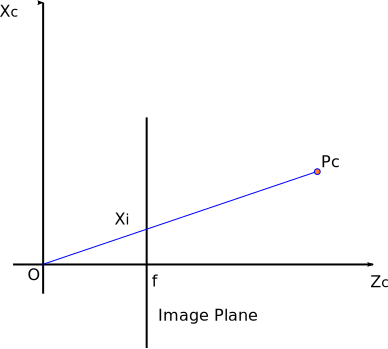
\includegraphics[width=0.7\textwidth]{pics/pinhole_model}
    \caption{Pinhole Camera Model showing two dimensions}
    \label{chap2:fig-pinholemodel}
\end{figure}

Figure \ref{chap2:fig-pinholemodel} shows the configuration with the pinhole located at
the origin and the image plane located at $f$, and the focal plane is parallel to the $x_i$
axis. The pinhole is often termed \emph{center of projection}. The $x$ axis of the image is located
upwards, while the real world $Z$ axis is the horizontal axis, that are called the
\emph{optical axis} or the \emph{principal axis}. This leads to the next parameters which
are needed to be defined.

The optical axis should ideally always be aligned with the center of projection. Due to
manufacturing inaccuracies this is rarely the case; therefor we need two parameters
to complete the pinhole model equations. These parameters are $c_x$ and $c_y$ which
describes the offset of the optical axis from the center of projection. Also the need for
different focal lengths in $x$ and $y$ might also be a necessity, because the individual
pixels on a typical low-cost image chip is often rectangular rather than square. Now the
equations relating real-world coordinates to image coordinates can be written.
\cite{openCV}
\begin{equation}
    \label{chap2:eq-pinhole}
    x_i = f_x \frac{X}{Z} + c_x \quad \quad y_i = f_y \frac{Y}{Z} + c_y
\end{equation}

The equations above are the \emph{projective} transformations, and are convenient to
write using homogeneous coordinates and arrange the parameters into a single $3\times 3$
matrix. This matrix is sometimes called the \emph{camera intrinsic} matrix. This has the
following form expressed in Homogeneous Transformation Coordinates. 
\begin{equation}
    M = \left[ \begin{matrix}
                f_x & 0 & c_x \\
                0 & f_y & c_y \\
                0 & 0 & 1 
                \end{matrix} \right]
\end{equation}
This is homogeneous representation of $\mathbb{R}^2$ represented in $\mathbb{R}^3$. To
recover to Equation \eqref{chap2:eq-pinhole} the results is divided by $w = Z$.

\paragraph{Lens Distortion}
\label{chap2:sec-distortion}
Because very little light goes through the pinhole, the pinhole camera is quite
impractical, therefor to make it practical for
real world use, lenses are introduced to bend, i.e. focus more light to the projective plane.
This allows for faster imaging of the world, but is also the source of more distortions
and inaccuracies. 

There are two types of lens distortions, \emph{radial} and \emph{tangential}. Radial
distortions are due to the construction of the lens, and most distortion occurs towards the edges of
the lens. This can be seen in pictures as ``barrel'' or ``fish-eye'' effects. 
These kinds of distortions are more present in cheap cameras which does not have the fancy lenses and optics
that the more high-end cameras have. There are also other types of lens distortions in imaging
systems, but they have typical lesser effects on the images, and will not be taken into
account. 

To model radial lens distortions the approach described by Brown in
\cite{lens-calibration} are used. The radial distortion is in practice small and can be
described by the two first terms of a Taylor series expansion around the center of the
lens. If the lens have high radial distortion, like fish-eye lenses a third term is
appended. The radial location of a point on the image plane can in general be described
like the equations below. 
\begin{equation}
\begin{aligned}
    x_{corrected} &= x_i ( 1 + k_1 r^2 + k_2 r^4 + k_3 r^6 ) \\
    y_{corrected} &= y_i ( 1 + k_1 r^2 + k_2 r^4 + k_3 r^6 ) 
\end{aligned}
\end{equation}
where $r^2 = x^2 + y^2$.

Tangential distortion is due to manufacturing inaccuracies and often causes the lens not to be
perfectly parallel to the imaging plane. The image might be deformed like a
trapezoid. This can be modelled by equations \eqref{chap2:eq-tangential-distortion}. The
derivation of these equations can be found in \cite{brown66}.
\begin{equation}
    \label{chap2:eq-tangential-distortion}
    \begin{aligned}
        x_{corrected} &= x_i + (2 p_1 y_i + p_2 (r^2 + 2 x_i^2)) \\
        y_{corrected} &= y_i + ( p_1 (r^2 + 2 y_i^2) + 2 p_2 x_i))
    \end{aligned}
\end{equation}
The parameters $p_1$ and $p_2$ are the tangential distortion parameters. These parameters
give enough information about the lens and camera to make corrections to the picture and
make the matching method easier, which of course will increase range accuracy. 

\begin{figure}[htbp]
    \centering
    \includegraphics[width=0.45\textwidth]{pics/left_tang_dist}
    \includegraphics[width=0.45\textwidth]{pics/right_tang_dist}
    \caption{The tangential distortion for the left and right camera of the Minoru 3D
    webcam}
    \label{chap2:fig-tang-dist}
\end{figure}
Figure \ref{chap2:fig-tang-dist} show a plot for the left and right camera of a stereo
rig. As seen from the figure, the cameras are supposed to be identical, but the tangential
distortion can be very different, and clearly show the need to estimate and rectify the
images. 


\paragraph{Epipolar Geometry}
To describe the stereo rig and geometry between the left and right cameras, the term
\emph{epipolar geometry} is introduced. Epipolar geometry exists between any two cameras.
The different center of projections, $C'$ and $C$, and corresponding
projective planes, $\Pi'$ and $\Pi$ and the term \emph{epipole} on the projective plane
$\Pi'$, $e'$ can now be defined as the image of the center of projection of the other 
camera, $C$. Suppose the point, $\mathbf{X}$ are viewed from both cameras, and have the image
location, $\mathbf{x'}$ and $\mathbf{x}$ in the left and right view, respectively. The line from the left
epipole, $e'$ to $\mathbf{x'}$ and the line from $e$ to $\mathbf{x}$ are called the \emph{epipolar
lines}. The planes made by the observed real world point, $\mathbf{X}$ and the center of
projections, $C'$ and $C$ are called the \emph{epipolar planes}, shown as gray planes in Figure
\ref{chap2:fig-epipolarGeometry}.
\begin{figure}[htbp]
    \centering
    \includegraphics[width=0.8\textwidth]{pics/epipolar}
    \caption{The epipolar geometry}
    \label{chap2:fig-epipolarGeometry}
\end{figure}

This allows for the following facts which simplify the computations and matching process
a great deal. 
\cite{epipolar}
\begin{itemize}
    \item Every 3D point in view of the cameras is constrained in an epipolar plane that
        intersects each image in an epipolar line.
    \item The \emph{epipolar constraint} says that a given feature in one image must lie
        along the corresponding epipolar line in the other view.
    \item The epipolar constraint means that the two-dimensional search for matching
        features simplifies to a one-dimensional search along the epipolar lines once the
        epipolar geometry of the stereo rig is known.
    \item The order is preserved. If two points are visible in both images and occur
        horizontally in that order in one image, they occur in the same order in the other
        image.
\end{itemize}

\paragraph{The Essential and Fundamental Matrices}
This matrices contains information about the translation and rotation which relate the
two cameras. The Essential matrix describes this translation and rotation in physical
space, and the Fundamental matrix also contains information about the intrinsics of the
two cameras, thereby describing the rotations and translations in pixel related
coordinates.

The derivation of the Essential matrix is interesting and is given here for reference.
Suppose a point $P$ related in the left camera coordinates, i.e. $P_l$ and the right
camera is located at $T$. The coordinates of $P_l$ in the right camera coordinates will
then be.
\begin{equation}
    \label{chap2:eq-Pr}
    P_r = R (P_l - T)
\end{equation}
Now, the epipolar plane is introduced. All points, $\mathbf{x}$ that lay on the plane with normal vector
$\mathbf{n}$ and passing through $\mathbf{a}$ obeys the equation,
\begin{equation*}
    (\mathbf{x} - \mathbf{a}) \cdot \mathbf{n} = 0
\end{equation*}
The cross product of $T$ and $P_l$ then becomes the normal vector of the epipolar plane,
because the epipolar plane includes both this vectors. Equation \eqref{chap2:eq-Pr} can be
rewritten as $P_l - T = R^{-1} P_r$ and including the cross product yields 
\begin{equation}
    (R^{-1} P_r)^T (T \times P_l) = 0
\end{equation}
The cross product can be expressed as a product between matrices by introducing the
skew-symmetric matrix $S$. \cite{modsim}
\begin{equation}
    S = \left [ \begin{array}{ccc}
                0 & -T_z & T_y \\
                T_z & 0 & -T_x \\
                -T_y & T_x & 0 \\ \end{array} \right]
\end{equation}
The essential matrix might now be defined, using $R^{-1} = R^T$ and moving it behind $P_r$.
\begin{equation}
    E = RS 
\end{equation}
which gives the equation
\begin{equation}
    \label{chap2:eq-fundamental}
    P_r^T E P_l = 0
\end{equation}
$P_r$ and $P_l$ are the real world 3D coordinates, and can be transformed to 2D
coordinates by the perspective transformation derived by the pinhole camera model. 

The relation between the Essential matrix and the Fundamental matrix can be showed with
help of the camera intrinsic matrix $M$, because we know that $q = Mp$, where $q$ are
pixel coordinates and $p$ is the 2D world coordinates. Substituting for $P$ in Equation
\eqref{chap2:eq-fundamental} gives: \cite{openCV}
\begin{equation}
    q_r^T(M_r^{-1})^T E M_l^{-1} q_l = 0
\end{equation}
The definition of the fundamental matrix, $F$ is then
\begin{equation}
    F = (M_r^{-1})^T E M_l^{-1}
\end{equation}
Both matrices are $3\times3$ and have rank two with seven parameters.


\paragraph{Finding Stereo Correspondences}
Now that the mathematics which describes points in the different views to each other, the
case of matching the corresponding points in the different view can begin. 
This is obviously only possible for visual areas that the two camera views overlap. 

There are couple of different matching algorithms. The most common are \emph{block
matching} algorithms. In \cite{konolige} a practical implementation of the block
matching algorithm is described. This algorithms use sum of absolute difference (SAD) windows to match 
points in the two views. This algorithm work only on undistorted, rectified, stereo
images. It first normalizes the image brightness which enhances textures. Then the search
for correspondences is carried out along the horizontal epipolar lines using the sum of
absolute difference window. After this the results are filtered to eliminate bad stereo
matches. This algorithm works best in highly textured environments, like outdoor
environments, and will prove less effective in structured surroundings like office
corridors and inside smooth pipelines. 

An extensive review of the different matching algorithms and their computational costs
can be seen in \cite{stereo-algorithms}.


\paragraph{Disparity and depth calculations}
When finally the stereo correspondences are found, the \emph{disparity} can be calculated.
The disparity is the difference in pixels coordinates from of the matched feature from one
image to the other. This disparity is inversely proportional to the depth. This means that
the depth perception of the stereo rig is better when relatively close to the cameras, as
Figure \ref{chap2:fig-disparity-depth} shows. 
Since the disparity is an integer, and the focal distance is assumed constant, 
the resolution of the Stereo Rig depends on the spatial resolution of the cameras and the 
baseline. The figure shows the depth-disparity plot with 6 different baselines, $20,
60, 100, 150, 200$ and $300$ millimetres. It is clearly seen that the depth resolution becomes better
when the baseline increases. 
\begin{figure}[htbp]
    \centering
    \includegraphics[width=0.7\textwidth]{pics/disparity}
    \caption{The relationship between depth and disparity}
    \label{chap2:fig-disparity-depth}
\end{figure}

Many robotic applications using stereo cameras utilize the disparity maps directly,
because they usually just require the detection of obstacles. 

The 3D coordinates of the point can be calculated from the disparities given by the
matching algorithms. This is the process of \emph{reprojection}. Using triangulation
between the two known camera locations the depth can be derived accordingly to 
\begin{equation}
    z = \frac{f T}{x_l - x_r}
\end{equation}

\subsubsection{Time-of-Flight Cameras}
The research and application of Time-of-Flight cameras have increased significantly during the last four
years. A Time-of-Flight camera is a compact device which makes it suitable to mount on
mobile platforms, and using it in navigation and localization applications. 

The most used ranging techniques by the cameras are \emph{intensity modulation} approaches and
\emph{optical shutter} technology. The first one is used by the best known manufacturers,
like MESA and PMD. The optical shutter approach is less expensive and has been used
by Zcam, which now have been sold to Microsoft. 


\paragraph{Intensity Modulation Approach}
\label{chap2:subsec-tof}
This approach uses modulated near infrared light (NIR) signal, $g$ which is reflected to and
captured by a CCD chip then correlated with the reference signal, $r$. 
\begin{equation}
    c(\tau) = g \otimes r = \lim_{T \rightarrow \inf} \int^{T/2}_{-T/2} g(t) r(t + \tau) dt
\end{equation}
where the signals, $g$ and $r$ might be
\begin{equation}
    g(t) = \cos{\omega t}, \quad \quad r(t) = b + a \cos{(\omega t + \phi)}
\end{equation}
where $\phi$ is the phase offset because of the travel time of the signal, $b$ is a
correlation bias, $a$ is the amplitude and $\omega$ is the modulation frequency. Solving
the integral yields 
\begin{equation}
    c(\tau) = \frac{a}{2} \cos{(\omega \tau + \phi )} + b
\end{equation}
which is the correlation function. 

The demodulation is usually done by sampling the correlation function at 4 equally spaced
phase offsets, and calculating the following relations
\begin{equation}
    \begin{aligned}
        \phi &= \tan^{-1} (\frac{A_3 - A_1}{A_0 - A_2}) \\
        I &= \frac{A_0 + A_1 + A_2 + A_3}{4} \\
        a &= \frac{\sqrt{(A_3 - A_1)^2 + (A_0 - A_2)^2}}{2}
    \end{aligned}
\end{equation}
where $A_i = c(i \frac{\pi}{2})$ for $ i = 0,..,3$ and $I$ is the intensity of the returned 
signal. From this the distance can be calculated using the phase delay $\phi$. 
\begin{equation}
    d = \frac{c}{4 \pi \omega} \phi
\end{equation}

There is a number of challenges when using this approach
\cite{time-of-flight-comp-graphics}
\begin{itemize}
    \item The resolution of the sensors are small compared to standard RGB or gray scale
        cameras. Current resolution on present day time-of-flight cameras is $204 \times
        204$. 
    \item ``Wiggling'' because of imperfections when creating the sinusoidal signals.
    \item Errors due to intensity measurements. Various sensor electronics might influence
        the measured intensity and give wrong readings.
    \item ``Flying Pixels'' occurs when a pixel in the camera oversees a region with
        large depth variances, e.g. at object boundaries.
    \item Motion artefacts might occur because the phase images are captured sequentially.
    \item Multiple reflections in highly reflective environments will cause erroneous
        distance measurements.
\end{itemize}

Standard lenses are used to capture the reflected light, which means that intrinsic
calibration should be carried out to specify the projection axis and distortion parameters
of the lens. The same approach as for standard cameras can be used. \cite{time-of-flight-comp-graphics}


\paragraph{Optical Shutter Approaches}
Light travels roughly at $c \approx 3 \times 10^8$ meters per seconds. This translates to
that light uses $6.7$ pico seconds to travel one millimetre. Imagine a light pulse emitted
at time $t$. This pulse travels in a spherical pattern and hits a 3D shape. The light wall
will be reflected back in a distorted pattern depending on the shape of the object.\cite{optical-shutter} 
A shutter in front of the CCD chip then
shuts out the rest of the light wall pattern. This will then produce a shape of the object
which can be used to calculate the distance, based on the times the shutter is open,
according to the following relation \cite{time-of-flight-comp-graphics}
\begin{equation}
    d = (1 - \alpha) d_{min} + \alpha d_{max}, \quad \quad \alpha =
    \frac{I_{gate}}{I_{total}}
\end{equation}
where $I_{gate}$ is the pixel intensity which arrives when the shutter is open, and
$I_{total}$ is the total amount of reflected light. Distances outside $d_{min}$ and
$d_{max}$ cannot be measured in the exposure. Therefore this technique requires multiple
exposures to get the desired depth resolution. The depth resolution of the cameras is 
clearly dependant on the achievable shutter speeds. 

This method is also prone to many of the challenges stated for the intensity modulation
approach.

\paragraph{3D camera calibration}
Some of the uncertainty and difficulties described above can be attenuated by properly
calibrating the Time-of-Flight sensor. Since the sensor uses a conventional lens to
capture the returned light, distortion due to the lens might occur. This can be calibrated
using the same method as for normal cameras, described in Section
\ref{chap2:sec-distortion}. 

Depth inaccuracies are present because generation of a perfect sinusoidal signal, which is
assumed for the correlation step, is not possible due to cost and hardware limitation. This
is the base for a systematic distance error, which when analyzed have a sinusoidal shape.
To correct this, the systematic error function is approximated using linear or higher-order 
polynomial models.  See \cite{tof-calibration} for more information.


\section{Map Data Representation}
\label{chap2:sec-representations}
The representation of sensor data is important for the functionality of the robot. This is
dependant on the amount of processing power and capacity that is available on the
implementation platform. 
The area which the robot is going to map is also of great importance when choosing the
representation. 

The major representation methods which is used in literature are summarized in the below
sections. There are two major ideas when it comes to map representation, 
metric and topological.

Metric representation uses the sensor data as we see it. It is the direct Cartesian
representation of the way the world is. Examples of this are CAD drawings of floor plans
and housing. These maps are often large and inexact, because of many kinds of
uncertainties.

A topological representation uses a more abstract approach. The world is represented by graphs,
which is nodes and links between them. This is a sparse and efficient way of representing
the world, but need more processing when the map is built. These kinds of maps are not
exact, because they are not expected to be. They simply describe the connection between
different kind of objects and the objects might have attributes describing how it really
looks. This method is useful in highly structured environments, such as pipelines, sewers,
and office landscapes, because the environments are somewhat predictable and easier to
recognize. 


\subsection{Occupancy Grid Maps}
Occupancy grid maps are a metric approach to the mapping problem and are widely used in 
robotic mapping, mostly because of it is simple to implement and use. It was developed 
by Elfes and Moravec in the mid 1980s, \cite{elfes}, \cite{moravec}. The method is quite 
robust and it is simple to implement with many kinds of sensors. Since this method is a
pure metric approach, it needs to know the robots position or pose, to create the map
correctly. 

This method divides the world into grids with probabilities that the grid is occupied. It
starts with all grids at 50 \%, equal probability that the space is occupied or not. As
the robot moves around it updates the grids according to its sensor readings. When for
example employing a laser range finder, the grid at the distance reported from the range
finder is marked as occupied according to some uncertainty set by the accuracy of the
range finder. The grids between the possible detected obstacles will then be decreased
because the probability of obstacles is less. 
\begin{figure}[htbp]
    \centering
    \includegraphics[width=0.7\textwidth]{pics/occupancy-grid}
    \caption{An example of the occupancy grid map}
    \label{chap2:fig-occupancy-grid}
\end{figure}

If the mission area is vast or three dimension grids are required, the occupancy gird maps 
are not the most computationally effective way to represent the world.
The representation is cumbersome and may lead to problems when dealing with
cyclic environments, because of the uncertainty in the sensor measurements and robots
pose and odometry. 


\subsection{Quad- and Oct-trees}
Quadtrees can be used to represent a 2D space by recursively dividing the space into
exactly four rectangles or squares. If this rectangles or squares do not include
interesting information then it will not be divided further. This dividing continues until
the smallest possible square, down to a certain value, is achieved. This creates a tree structure which is easily
traversed and searched if necessary. An \emph{Oct-tree} is the same only each node has 
eight child nodes instead. This can be used to represent 3D spaces, see Figure
\ref{chap2:fig-octtree}.
\begin{figure}[htbp]
    \centering
   \includegraphics[width=0.5\textwidth]{pics/octtree}
    \caption{A Quadtree representation}
    \label{chap2:fig-octtree}
\end{figure}
\cite{mathisen}


\subsection{Topological Maps}
Object maps are topological maps and represent the sensed world in the form of predefined nodes and links
between them. Each node has a set of attributes, like length, links to doors etc. This is
a compact way to express the world and is much more computationally effective with larger
maps than the occupancy grid maps might be. Examples of such nodes are corridors,
junctions and dead ends, but these nodes must be suited to the application of the robot.
Depending on the environment to map, the nodes might be different geometrical primitives,
like cylinders, planes, lines, or arcs. 

The map of the London Underground is a common every day example of a topological map. It describes
the important things as stations, but not the geometrical distances which are not important
when navigating the London Underground. \cite{thrun}


\subsection{Mixed Approaches}
This is when you take the best of both worlds. The easy and effective way of the metric
maps, mixed with the abstract topological maps. This will help reduce the size of
the maps in the robots memory, and also make it more computationally effective because the
maps are sparse. 

This uses 
the metric approach for the rooms that have a lot of details, chairs, desks etc. and for
corridors and less detailed areas the topological approach, when the metric and
geographical information are not that important. 
\cite{thrun}

%\section{Sensor Fusion Techniques}
%Multi sensor fusion has been a target for much research. The topic seeks to combine the
%abilities of several sensors and sensor types, to make the combined result better. 


%According to \cite{sensor-fusion-mobile-robots} there is a lot of ways to achieve sensor
%fusion in mobile robotics. The use of multiple sensors is favorable because the readings
%can be fused to make a better estimate of the current situation. 

%Multi sensor fusion is widely used in robotics today. This because it allows the designer
%to use different measurement principles which have different capabilities. 


%\subsection{Low-level Fusion}
%The term low-level fusion is often used when the sensor data is directly integrated
%resulting in parameters and state estimates of the model. These methods are mostly purely
%mathematical. This method involves the Kalman Filter, and other Bayesian approaches. In
%many cases \'a priori information are used to verify or improve the
%estimates from the sensors.

%These methods are probabilistic and require that you know something about the
%statistical properties of the sensors and the \'a priori model. 



\section{Feature Extraction}
\label{chap2:sec-feature-extraction}
The need for feature extraction should be obvious when dealing with autonomous robot
navigation. For the robot to know where it is it needs to recognize its surroundings. This
is a difficult step, because computers are not good at this, as the human
brain is. 

By feature extraction means to find interesting objects in a dataset. The difficulty of
this varies with the size of the dataset and amount of noise polluting the set.

This problem is relaxed a bit when the surroundings are confined to pipelines, because the
environment is made up of known parts, that can be included in a database which the
sensor data can be matched to. 
By feature extraction in this report the meaning is to recognize the different types of junctions
that the robot will travel through. 

Standard fitting techniques assumes the whole dataset is a part of the model when fitting
a model to it. This
means that it assumes that errors and ``wild points'' in the dataset can be averaged out.
Said in another way, the correctness of the dataset is a function of the size of the
dataset. When for example in computer vision, graphical primitives such as planes, and
cylinders are in the same scene, it is difficult to know which points in the dataset
correspond to which graphical primitive. Therefore, one will need to sort out which points
``belong'' to the different primitives. If a least-squares approach is used the fitting
procedure to the primitives would not be very successful because this method will assume
that all points have some relation to the fitted primitive. \cite{ransac}

A data set might be consisting of many different features that cannot be detected unless
the dataset is segmented in some way. This means finding a subset of the original dataset
only including the points which belong to the features being extracted. 
When the subsets are extracted the parameters of the features can be estimated. 


\subsection{Point Feature Histograms}
Point feature histograms are a way of assessing the local geometry around a point in a
3D point cloud. This can be used to segment the point cloud into given geometrical
primitives. The computation of a point feature histogram works as follows, for each point
$p$, all of $p$'s neighbours inside a sphere with radius $r$ are selected. For every pair
of points in the selected subset the normals $n_i$ and $n_j$ are estimated. A Darboux
$uvn$ frame is defined according to 
\begin{equation}
    u = n_i, \quad v = (p_j - p_i)\times u, \quad w = u \times v
\end{equation}
The following angular variations are then used for categorizing the points. \cite{pfh}
\begin{equation}
    \begin{aligned}
        \alpha &= v \cdot n_j \\
        \phi &= (u \cdot (p_j - p_i)) / || p_j - p_i|| \\
        \theta &= \arctan (w \cdot n_j, u \cdot n_j)
    \end{aligned}
\end{equation}
These angular variations are sorted into histogram bins according to 
\begin{equation}
    idx = \sum_{i=0}^{i \leq 2} \left [ \frac{f_i \cdot d}{f_{i_{max}} - f_{i_{min}}}
    \right] \cdot d^i
\end{equation}
where $idx$ is the point feature histogram bin index, $d$ is the number of subdivision of
the features maximum theoretical value range $(f_{i_{max}} - f_{i_{min}})$. This will sort
the points into bins according to how the angular variations vary. 

Different geometric surface primitives have different signatures. \cite{pfh-geometric}
shows the distinct histogram formation for convex surfaces as cones, spheres, cylinders
and planes. This can be used to classify points and thereby isolating important features
in the scene. 

\cite{pfh-segmenting} uses a combination of local fast point feature histograms to segment
the object of interests into geometric primitives, then a global version of the point
feature histogram are employed to detect and categorize objects in the given scene. The
shown results are promising. 

\subsection{Surface Fit Algorithms}
\label{chap2:sec-surface-fit-alg}
Suppose a point on a 3D surface can be expressed as
\begin{equation}
    \mathbf{x} = f(\mathbf{s}, t)
\end{equation}
$\mathbf{s}$ is a parameter of size $p$ characterizing the nature of the surface, i.e. the
radius of a circle. $t$ is the positional parameters which fixes the position of the point
on the surface. For a sphere, the parameters vector, $\mathbf{s}$ would have four parameters,
the three dimensional position and the radius, while the $t$-vector would have 2
parameters representing the angles around two of the axes, in this case the spherical
coordinates.

The surface fit problem can be sated as a minimization problem. The
objective function to be minimized is then the distance from the data set to a cylinder
surface. The distance can be given as 
\begin{equation}
    d( \mathbf{s}, \mathbf{p})  = | ( \mathbf{p} - (\sigma + \frac{1}{k} \mathbf{n})
    \times \mathbf{a})| - \frac{1}{k}
\end{equation}
$\mathbf{p}$ is an arbitrary point, $\sigma \mathbf{n}$ is the point which is the closest
point on the cylinder to the origin, $\frac{1}{k}$ is the radius of the cylinder, and $\mathbf{a}$ is the
direction vector of the cylinder. $\mathbf{n}$ obeys the relation $\mathbf{a} \cdot
\mathbf{n} = 0$. 

\cite{ls-fit-cylinder} proposes to use an approximation to the distance, both because it
simplifies and the computational difficulties because of the square root vanishes, but
also to avoid computational singularities when calculating the distance. The proposed
expression to be minimized then becomes
\begin{equation}
    \tilde{d} = \frac{k}{2} |\hat{\mathbf{p}} \times \mathbf{a} | ^2 - \hat{\mathbf{p}} \cdot
    \mathbf{n}
\end{equation}
where $\hat{\mathbf{p}} = \mathbf{p} - \sigma \mathbf{n}$. This distance is robust to
mathematical singularities and is less computationally intensive than taking the square
root of something. The function which is to be minimized then becomes
\begin{equation}
    \label{chap2:eq-ls-cylinder-min}
    \sum_i \tilde{d}^2(\mathbf{s}, \mathbf{p}_i)
\end{equation}
The cylinder can be completely described and parametrized with the \emph{direction cosines} the radius, and
the position of the axis. The various minimization algorithms can be used and will be
discussed in the next section.


\subsubsection{Leasts-Squares Gauss-Newton Optimization}
\label{chap2:subsec-gauss-newton}
Least-squares method is a common way to optimize and fit data sets to a proposed model.
The idea is to minimize the objective function 
\begin{equation}
    f(x) = \frac{1}{2} \sum_{j = 1}^m r^2_j (x)
\end{equation}
where the $r_j(x) \in \mathbb{R}^n \rightarrow \mathbb{R}$ is called the \emph{residual} and
is generally a linear or nonlinear function. This function can be written as a vector then
the Jacobian can be defined as
\begin{equation}
    J (x) = \left[ \frac{\partial r_j}{\partial x_i} \right]
\end{equation}
The Jacobian is a $m \times n$-matrix. Using this the Hessian, i.e. the second order
derivative of $f$ can be expressed as
\begin{align}
    \nabla f(x) &= \sum_{j = 1}^m r_j(x) \nabla r_j(x) = J(x)^T r(x) \\
    \nabla^2 f(x) &= \sum_{j=1}^m \nabla r_j (x) \nabla r_j(x)Å T + \sum_{j=0}^m r_j(x)
    \nabla^2 r_j(x) = J(x)^T J(x) + \sum_{j= 0}^m r_j(x) \nabla^2 r_j(x)
    \label{chap2:eq-hessian}
\end{align}
This allows for the Hessian, which usually is very cumbersome and computationally
intensive to calculate, to be approximated by the Jacobian. This is especially true when
the residual terms are small, then the first term in Equation \eqref{chap2:eq-hession}
will dominate the expression. 

The Gauss-Newton method is a modified Newton method that uses line search to find the
best fit. Standard Newton methods are based on solving $\nabla^2 f(x_k) p = -\nabla
f(x_k)$ with regard to $p$ to find the search direction. The Gauss-Newton approach uses
the approximation $\nabla^2 f_k \approx  J_k^T J_k$, which gives the following equation to
solve
\begin{equation}
    J_k^T J_k p_k = - J_k^T r_k
\end{equation}
The approximation of the Hessian saves quite a lot computational time and the impact on
the direction is not that great. Also, around the solution $x^*$ the first term in
\eqref{chap2:eq-hessian} will dominate the other factors. This will cause the convergence
rate of the algorithm to be equal to those of the standard Newton methods, which is
quadratically when close to the solution $x^*$.\cite{optreg} 

$p_k$ is guaranteed to be a descent direction when $J_k$ has full row rank and the
gradient $\nabla f_k$ is nonzero. The Gauss-Newton also has the advantage that the
nonlinear objective function might be divided into linear subproblems and solved
individually. This means that the search direction, $p_k$ is the solution of
\begin{equation}
    \min{p} \frac{1}{2} || J_k p + r_k ||^2
\end{equation}

The term which is minimized is \eqref{chap2:eq-ls-cylinder-min} subject to the direction
of the cylinder axis, the radius and the start position center of the axis. 


\subsubsection{RANSAC Algorithm}
RANSAC is an acronym of \emph{RANdom SAmple Concensus}. This algorithm is a
non-deterministic algorithm which is robust to ``wild points'' in the dataset. This is
practical when the datasets are polluted with noise and measurement errors.
The RANSAC algorithm is basically a two step process, which is repeated until some
criterion is fulfilled. The first step is called the \emph{hypothesize}-step which selects
the \emph{minimal sample set} (MSS). This is the absolute minimum required to represent
the fitted model, i.e. for a 2D line, two points are needed to uniquely define the
line. The model parameters are computed using only the points from the MSS.

The next step is the \emph{test}-step, which determines the amount of points from the
whole dataset which are consistent with the parameters computed from the MSS set. This set
of points is called the \emph{consensus set} (CS). The algorithms search for points and
terminates when the probability of generating a better consensus set drops below a certain threshold, i.e.
no more points can be added to the consensus set. The distance from the points in CS to the 
fitted model is used as a measure on how good the model is. This model is kept as the best
fit up to date. \cite{ransac-dummies}

This is done a finite number of times and dependant on the number of \emph{inliers}, i.e.
a point that are defined to belong to the model, the model is compared to the present best
fit, or rejected.

To ensure that RANSAC gives the best fit model, the number of iterations to find the best
fit must be large enough. Since the selection of the initial MSS is done randomly, one
cannot guarantee that the MSS only consists of inlier points. The probability of
selecting $h$ sets which are polluted by \emph{outliers} is $(1 - q)^h$, where $q$ is the
probability of selecting an inlier from the dataset. The idea is to pick a $h$ large enough that the
probability that all the sets are contaminated by outliers will be lower than a certain
value, $\epsilon$ called the \emph{alarm rate}, $(1 - q)^h \leq \epsilon$. Reorganizing
this to find the number of iterations gives
\begin{equation}
    \hat{T}_{iter} = \left \lceil \frac{\log \epsilon}{\log (1 - q)} \right\rceil
\end{equation}
In general the number $q$ is difficult to calculate, according to \cite{ransac-dummies}
the probability can be approximated by 
\begin{equation}
    q = \prod_{i = 0}^{k-1} \frac{N_I - i}{N - i} \approx \left ( \frac{N_i}{N} \right)^k
\end{equation}
where $N_I$ is the total number of inilers, $N$ is the total number of points in the
dataset, and $k$ is the number of times one will try to pick a set of inliers. This is a
valid approximation because $k$ most probably is much smaller than both $N$ and $N_I$. A
estimate of the number of inliers can be found, using the number of inliers found
up-to-date. \cite{ransac-dummies}


\section{State-of-the-Art Pipe Inspection Robots}
\label{chap2:sec-state-of-the-art}
To get an overview of other similar project, the next section will give an introduction to
other research projects concerning pipe and sewer inspection robots, travelling inside the
pipes. 

The German MAKRO project \cite{MAKRO-project} uses a multi-segmented robot, each segment 
having three degrees of freedom, panning, tilting and rotation. This is a complete
research project to create a fully autonomous sewer inspection robot. The robot is
equipped with various sensors including, a stereo camera rig for dense stereo
reconstruction of the pipe structure. Proximity IR sensors directed perpendicular to the
motion axis to sense the pipe walls, and an ultrasound sensor directed forward for
position measurements. An experimental set-up with a laser to project a predetermined
pattern on the surroundings together with one of the cameras to calculate the direction of
th sewer pipe axis. The control system is based on an AI machine learning method called \emph{Q-Learning}, in
a closed-loop, hierarchical fashion.


\cite{MRINSPECT-V} proposes a method of visual landmark recognition by using shadows
generated by a special illuminator. The method where implemented on \emph{MRINSPECT V}, a
four-segmented robot, where two modules are driving modules with four wheels presented at
120 degrees interval around the module, one at the front and one at the end. The two
remaining modules contains the batteries and control modules. 
The captured images from a camera is filtered and the
shadows are extracted using a binarization and thresholding approach. The shadow profiles are
labelled with unique ID-tags and the center of the shadow are calculated. Depending on
where the shadows are cast, the direction of the pipe feature can be determined. The
shadow pattern is matched against a database to determine what kind of profile the robot
are going trough. The shadow detection system is used to locate profiles and term them as
landmarks. When the robot is going through the landmark, a 2-axis gyro and odometry of
the wheels are used to determine the direction and length of the landmark and updating
this to the internal landmark database. When the robot has passed the landmark, the 
landmark search using shadows are restarted. This method was tested on a 8 inch (20 cm)
gas-pipeline structure, with L-shaped and T-shaped junctions arranged in a 3D dimensional
arrangement and showed promising results. 


\emph{Kario-II} is a multi-segmented robot, typically made up of 6 drive segments with
active wheels and 5 joints between these segments which each have 3 degrees of freedom,
making a total of 21 degrees of freedom of the robot. \cite{Kairo-II} provides a control
strategy of controlling and path planning for the full 21 DOF model in unstructured and
dynamic environments. An algorithm called the \emph{virtual tube} is developed for
navigating in complex environments. No field tests have been preformed yet, and there is
still much work to be done for this robot to be able to inspect real world environments. 


\cite{KANTARO} describes \emph{KANTARO}, a single segement, sewer-pipe inspection robot 
capable of moving autonomously in 200-300 mm pipes. The robot turns smoothly in 90 degrees 
junctions and able to go down 5 cm steps. The robot consists of a platform of 4 wheels,
and a payload box placed on top. The robot is equipped with a CCD camera with ``fish eye''
lens and proper lighting together with a laser scanner. This laser scanner is custom made
and uses the optical triangulation principle and produces measurements with accuracy
of about 1 mm. KANTARO have been tested in a dry sewer test environment, traversing
L-bends and T-junctions with high stability, according to the authors. But much work is still
to be done with regard to make this robot robust enough for the real world. 


\cite{sintef-tof} uses a Time-of-flight camera mounted on the Pipe Inspection Konda. It
uses the M-SAC criterion to fit a cylinder or a cone to the sensor output of the
time-of-flight camera. The cone was used instead, because experiments showed that it gave
a better fit to the dataset. The system then uses the difference between the fitted
cylinder or cone and
a ideally synthesized image of the scene to find junctions and other things worth noting.
The system is implemented with obstacle avoidance and gives promising results. This report
is loosely based on the method described in the article. 





%file included in thesis.tex


\chapter{Sensors}
\label{chap3-sensors}

\section{Comparisons Between the Proposed Sensors}
For this project, some of the sensors was not decided. This gave the ability to chose a
sensor, based on cost, resolution, accuracy and delivery date. The manufacturers that were
considered where the Japanese \emph{Hokuyo} and American \emph{SICK}. This two companies are to the
authors knowledge the leading manufacturers of laser range finders, small enough to be
mounted on small robotic platforms. The various models and key parameters are summarized
in Table \ref{chap3:tab-sensors}.
\begin{table}[htbp]
    \begin{tabular}{|c|c|c|c|c|c|}
        \hline
        Sensor              & LMS-100 & LMS-200 & UTM-30LX & URG-04LX & URG-04LX-URG01 \\
        \hline
        Max Range           & 20 m    & 80 m    & 30 m     & 4 m      & 5.6 m          \\
        Accuracy            & 12 mm   & 30 mm   & 30 mm    & 10 mm    & 30 mm          \\
        Field-of-View       & $270^\circ$ &$180^\circ$  & $270^\circ$ & $240^\circ$ & $240^\circ$  \\
        Angular Resolution  & $0.25-0.5^\circ$  & $0.25-1^\circ$ & $0.25^\circ$ & $0.36^\circ$ & $0.36^\circ$  \\
        Scan Frequency      & 50 Hz   & 75 Hz   &  40 Hz   & 10 Hz    & 10 Hz          \\
        Weight              & 1.1 Kg  & 4.5 Kg  & 210 g    & 160 g    & 160 g          \\
        Power Consumption   & Not Specified & Not Specified  & $<8 $ W & $~2.5$W  &$~2.5$W  \\
        \hline
        Cost                & \$5500  & \$5000  & \$5000   & \$2400   & \$1100         \\
        \hline
    \end{tabular}
    \caption{Comparison between the proposed sensors}
    \label{chap3:tab-sensors}
\end{table}

The LMS-100 and LMS-200 are relatively large sensors compared to the ones from Hokuyo. The
scanning frequency of the SICK range finders are quicker, but because PiKo is not that
fast and taken into account that the 3D sensor which will have much greater scanning
frequency. This means that the frequency of the 2D sensor is not that important. The most
important thing is that it is as accurate as possible. Also, the Hokuyo sensors are much
cheaper than the ones from SICK which gives them the advantage.

Because of favourable size, weight, accuracy and cost the Hokuyo \emph{URG-04LX} was
chosen. The sensor will be discussed in Section \ref{chap3:sec-urg}.

\subsection{3D Sensors}
There are many different depth sensors available at the consumer market. This section will
outline some of them, and describe the \emph{MESA Imagining} SR-3000 in more detail.
The development of depth-sensing cameras and devices have accelerated the last years
because of the increased computational ability and the fact that electronics become
cheaper and cheaper. \cite{low-cost-depthcameras}

During the next years the video game industry most certainly will
incorporate this new technology into video games to take the games to a new level, such as
Microsofts \emph{Project Natal} for Xbox 360 \cite{project-natal}. This uses infrared
projected light stereo. The camera will sense depth by using stereo cameras to sense a
coded near-infrared light pattern, by using standard CMOS image sensors. According to
Microsoft the accuracy in depth will be about 1 cm, and practical ranges will be about
1 to 3.5 meters. The camera will operate at 640x480 pixel resolution at 60 Hz
\cite{conceivably-tech}.



\section{Laser Range Finder Hokuyo URG-04LX}
\label{chap3:sec-urg}
The laser range finder which were selected to this application was the \emph{Hokuyo
URG-04X}. It uses an infrared laser to sweep a view field of $240^\circ$ ten times a
second. The full $360^\circ$ circle are segmented using ten bit, which gives angular
resolution of $\frac{360}{2^{10}} = 0.3515$. The ranges have twelve bit resolution, each
bit representing a millimeter, which gives the total measurable length of $2^{12} = 4096$.
\begin{figure}[htbp]
    \centering
   % \includegraphics[width=0.7\textwidth]{pics/lrf-urg}
    \caption{The Hokuyo URG-04X}
    \label{chap3:fig-urg}
\end{figure}
The effective area which gives range readings are the sector form the 44th step to
725th step, where the sector starts at $60^\circ$ if zero degrees is right backwards. See
Figure \ref{chap3:fig-urg-sector}.
\begin{figure}[htbp]
    \centering
    %\includegraphics[widht=0.7\textwidth]{pics/urg-sector}
    \caption{The sweep sector of the URG-04X}
    \label{chap3:fig-urg-sector}
\end{figure}

The sensor can not measure below 20 mm because it is not practical, and the range codes
from 0--19 are error codes. The codes can describe if the intensity of the reflected light
is too low or too high which indicates erroneous results. A detailed summary of the
error codes and what they mean can be found in Appendix \ref{app:urg-error}.


\subsection{Noise- and Error Sources}
Major error sources of the URG where discussed in Section \ref{chap2:lrf-error}. It is
possible to read both range and intensity of the reflected signal from the URG. The
intensity can be used as a quality control of the range value. 





\section{Stereo Camera Minoru 3D WebCam}


\subsection{Camera Calibration}
To work with stereo images the captured images need to be rectified, i.e. the images need
to be corrected for distortion introduced by the camera lenses. This is a part of
calibrating the camera, meaning that the intrinsic parameters of the camera are
determined and the lens distortion parameters described in Chapter \ref{chap2}.

To determine the parameters the \emph{Camera Calibration Toolbox} for Matlab is used
\cite{camera-calib-toolbox}. 20 image pairs are captured of a checker board in various
distances and orientation from the stereo rig. This images for left and right camera are
processed individually to calculate the distortions of the individual camera. 
\begin{figure}[htbp]
    \centering
    \includegraphics[width=0.8\textwidth]{pics/left7}
    \caption{Seventh left image in the calibration sequence}
    \label{chap2:fig-checkerboard}
\end{figure}
The four extreme-most corners of the checkerboard is selected in each image, and an
internal algorithm detects the corners of the squares in each image. This gives an initial
guess on how the distortion parameters are. The reprojection error is then minimized with
regard to the distortion parameters using a nonlinear gradient decent algorithm. For more
information on how this is carried out, see \cite{heikkila}.

The distortion parameters for both cameras are summarized in Table
\ref{chap3:tab-distortion-coeffs}.
\begin{table}
  \centering
    \begin{tabular}{|c|c|c|} 
        \hline
                & Left Camera       & Right Camera \\
        \hline
        $k_1$   & $-0.10292 \pm 0.3794$            & $-0.5450 \pm 0.02456$  \\
        $k_2$   & $-0.22555 \pm 0.49387$            & $-0.38334 \pm 0.13037$  \\
        $h_3$   & $ 0$                          & $0$                  \\
        \hline
        $p_1$   & $-0.00361 \pm 0.00141$    & $-0.00033 \pm 0.00115$ \\
        $p_2$   & $0.00206 \pm 0.00174$     & $ 0.000491 \pm 0.00243$  \\
        \hline
    \end{tabular}
    \caption{The distortion parameters discussed in Section \ref{chap2:sec-distortion}}
    \label{chap3:tab-distortion-coeffs}
\end{table}





Figure \ref{chap3:fig-comp-lensdist} below shows how the camera lenses of the Stereo camera distorts the pictures
towards the edges of the lens. 
\begin{figure}[htbp]
    \centering
    \includegraphics[width=0.47\textwidth]{pics/left_comp_dist}
    \includegraphics[width=0.47\textwidth]{pics/right_comp_dist}
    \caption{The left and right camera distortion due to lens nonlinearities}
    \label{chap3:fig-comp-lensdist}
\end{figure}
The Figure clearly shows that the principal axis are offset from the center of the images,
and that it is opposite for the left and right images. This means that the view field of
the two cameras will be quite different, and result in a reduced field-of-view for the
total stereo rig.

The intrinsic parameters for the cameras are summarized in Table
\ref{chap3:tab-intrinsic-stereo}. The values are all in pixel coordinates. The real focal
distances can be calculated by knowing the pixel-to-length ratio.
\begin{table}
  \centering
    \begin{tabular}{|c|c|c|} 
        \hline
                & Left Camera       & Right Camera \\
        \hline
        $f_x$   & $877.11\pm 2.94$  & $880.28\pm 3.08$  \\
        $f_y$   & $876.49\pm 2.88$  & $879.20\pm 2.96$  \\
        \hline
        $c_x$   & $350.00\pm 6.32$  & $338.54\pm 6.21$ \\
        $c_y$   & $214.30\pm 4.65$ & $267.59\pm 4.35$  \\
        \hline
    \end{tabular}
    \caption{Intrinsic parameters of the stereo rig in pixel related units including
    uncertainties}
    \label{chap3:tab-intrinsic-stereo}
\end{table}
The focus distances in the x and y-direction are slightly different in both cameras. This
suggests that the pixels of two cameras are not exactly square. The principal axis in both
cameras are also in very different places. This is problematic because a stereo rig should
be horizontally aligned to give the best results. Because for the off-center principal
axis the field-of-view of the stereo rig will be quite reduced.


This distortion can be removed and are called rectifying the image. This makes common
features in the two images aligned horizontally. This makes it much easier for the matching
algorithm because it only need to match vertically.


\subsection{Depth resolution}
The depth resolution which can be expected from the Stereo cam are,
\begin{equation}
    \Delta Z = \frac{Z^2}{f T}\Delta d
\end{equation}
where $\Delta d$ is the smallest increment in disparity, $f$ is the focal distance, and
$T$ is the baseline. This is determined in the implementation in this case the OpenCV
library. This is useful when calibrating the stereo rig, and when testing the program,
because it tells what kind of ranges one can expect from the rig.


\subsection{Noise- and Error Sources}
The major source of errors connected with stereo cameras are bad feature matches. This
will cause bogus distances. This is heavily correlated with the amount of noise captured
by the imaging sensors and other disturbances.




\section{Time-of-Flight Camera MESA SwissRanger-3000}
The time of flight camera gsjekkives out either Cartesian coordinates or intensity. This
intensity is the amplitude of the returned laser light. Figure
\ref{chap3:fig-tof-amppicture} shows a typical amplitude plot of the inside of a pipe.
\begin{figure}[htbp]
    \centering
   % \includegraphics[width=0.8\textwidth]{pics/tof-amppicture}
    \caption{Typical amplitude image of the SR-3000 ToF-camera}
    \label{chap3:fig-tof-amppicture}
\end{figure}


\subsection{Intrinsic Parameter Calibration}


\subsection{Depth Calibration}


\subsection{Noise- and Error Sources}






\section{Sensor Configurations}
There are a couple of possible sensor configurations available for this project. ***SHOULD
MAYBE BE IN THE IMPLEMENTATION CHAPTER?****

The Laser Range Finder should alway be used in every sensor configuration. This should be
the primary source of length measurements since this is the most accurate of all the range
devices. 

The stereo camera might be looked upon as a cheap type of the Time-of-Flight camera. So
the two possible configurations are:
\begin{itemize}
    \item Laser Range Finder and Stereo Camera
    \item Laser Range Finder and Time-of-Flight Camera
\end{itemize}
The Stereo Camera will give sparse range data, while the Time-of-Flight camera will give
dense range data. 







\chapter{Sensor Fusion}
Multi sensor fusion is an important aspect when it comes to large systems. This because it
can provide extra resolution or better estimates of the current situation. The need for
this when the systems are big and complex are obvious. But this is also important in
smaller systems. This gives the system abilities to ``feel'' more of its surroundings
without user input. ************!!!!!!!!!!!************


\section{Kalman Filter}


\section{Other Sensor Fusion Techniques}






%file included in thesis.tex


\chapter{Data Representation}
\label{chap5}
This section will describe the world representation used in the implementation.

\section{World Representation}
The world representation should have a number of qualities. First it must represent the
world in a satisfactory way. It should be easy to update and take up as little memory in
the robots memory as possible. Third it should be easy to understand for a human operator
without too much post-processing. 

When choosing how to represent the world one must take into account how much reasoning and
processing the robot should do with the sensor data. The more abstract world
representation, the more reasoning and processing must be done at the robot. On the
upside, abstract representations takes up less space in memory, and can be more
computationally effective when it comes to path finding and planning, than the less
abstract map representations. 

The problem when a robot has to reason, is that it might take the wrong decisions, and the
risk of erroneous map making are high. 

\subsection{Nodes}
The representation in this project is a kind of topological map. It is abstract in the way
that the world are classified into given nodes. Known features of the world are recognized
and represented as nodes in a graph. 

This means that the world need to be classified into predefined nodes before the mission
is started. In this project the nodes are junctions, or bends that are easily recognized
because of their fundamental difference to the straight pipe segments. 

The nodes should have a number of attributes describing how the node is different from the
other nodes. These attributes are:
\begin{itemize}
    \item Node type
    \item Number
    \item Time stamp when discovered
    \item Previous Node
    \item Distance since last node
    \item Orientation
    \item Number of edges and the angles of those
    \item List of anomalies
\end{itemize}

Most of this attributes are self-explaining, but the last attribute, \emph{list of
anomalies} deserves a closer explanation. 

Anomalies are those things that the robot should look after, and record. An anomaly are
everything that is not expected. In a pipe environment the surroundings are assumed to be
in some way, because they are designed that way. Everything that is not as expected should
be recorded for later inspections. 

This list will contain every anomaly from the previous node to the next one, where the
list is stored. The list will contain a time stamp of when it was discovered, distance
traveled from the previous node, and a remark why it was detected as an anomaly. 

Since the anomalies will be detected before the node which will contain the list are
detected, the list is temporary stored in the robots memory until the next node are
detected. 


\section{Map-building From the Sensor Data}


\subsection{Cylinder Fit from 3D Sensor Data}
The cylinder fit is a Least-Squares Gauss-Newton algorithm. This algorithm are very
useful since it does not require the calculation of the Second order derivatives, or the
Hessian matrix. This calculations are very cumbersome and computationally expensive. 

The point cloud from the Time-of-Flight camera are divided into equally spaced
sections with regard to the z-axis, i.e. the depth into the pipe. This intervals of 3D
data are fed into the algorithm and produces a set of cylinders which are fitted to the
pipe. The distance of the points from the proposed cylinder are output from the algorithm
and can be used for determining if the cylinder fit is a good fit. 
\begin{algorithm}
    \caption{Cylinder Fit Algorithm}
    \label{chap5:alg-cylinderfit}
    \begin{algorithmic}
        \REQUIRE (X, Y, Z) $\leftarrow$ point cloud
        \STATE Average point cloud over $n$ samples
        \STATE Remove all trivial points
        \STATE Sort on Z-coordinate
        \STATE Divide point cloud into $n$ equally spaced $SubSets$ according to $|Z| >$
        Threshold
        \FOR{every $SubSets$}
            \STATE Get initial values for Surface Fit algorithm
            \STATE  $r, a, x_0, d$ $\leftarrow$ run surface fit algorithm on $SubSets$
            with given Initial Values
        \ENDFOR
        \FOR{every $r$}
            \IF {$r > m \times PipeRadius$}
                \STATE Mark $r$ as erroneous
            \ENDIF
        \ENDFOR
    \end{algorithmic}
\end{algorithm}

\begin{figure}[htbp]
    \centering
    %\includegraphics[width=0.7\textwidth]{pics/cylinderfit}
    \caption{The set of cylinders fitted to the point cloud}
    \label{chap5:fig-cylinderfit}
\end{figure}
An example of a set of fitted cylinders are shown in Figure \ref{chap5:fig-cylinderfit}.
One might see that the axis are off. This is because noise and the least squares nature of
the fit. The noisy points will draw the cylinder off axis compared to the real one. 

The user parameters in this algorithm are the \emph{subset threshold} which decides the interval
of the subsets and also how many cylinders should be fitted to the given point cloud. The
other parameters are $m$ which tells for which values the predicted cylinder radii are
erroneous. 

The initial values which are required for the surface fit, is the assumed start position
of the cylinder which at the first \emph{SubSet} is at the origin with regard to the
ToF-camera sensor frame, and the initial axis which unless other is said is along the
z-axis, i.e. into the pipe seen from the camera.


\subsection{Line Fit and Arc Fit in 2D Sensor Data}
Line fit algorithm is a least-squares line fit algorithm. For this to work properly, a
selection of points assumed belonging to the line need to be fed into the algorithm. To
select this points a histogram is formed for both x- and y-direction of the points. This
will detect points which lie in a horizontal- and vertical lines. This points are selected
and fed into the line fit algorithm. 

This method involves a number of parameters and threshold values which need to be set and
tuned by the user. 



\section{Positioning in the World Representation}







%file included in thesis.tex


\chapter{Implementation}





\chapter{Testing}


\section{Test Environment}


\section{Test Results}






\chapter{Discussion}
This chapter will evaluate how the implemented algorithms work, the shortcomings and
possible solutions to problems. 

\section{How did it perform?}
How the system preformed are outlined in this section. Starting off with the
\emph{SwissRanger 3000} Time-of-Flight camera. 

\section{Why did it perform this way?}







\chapter{Conclusions}


\section{Further Work}






%\language{english}

% sets line spacing
\renewcommand\baselinestretch{1.2}
\baselineskip=18pt plus1pt



% --------------------------------------------------------------
%:                  BACK MATTER: appendices, refs,..
% --------------------------------------------------------------

% the back matter: appendix and references close the thesis


%: ----------------------- bibliography ------------------------

% The section below defines how references are listed and formatted
% The default below is 2 columns, small font, complete author names.
% Entries are also linked back to the page number in the text and to external URL if provided in the BibTex file.


% PhDbiblio-url2 = names small caps, title bold & hyperlinked, link to page 
\begin{multicols}{2} % \begin{multicols}{ # columns}[ header text][ space]
\begin{tiny} % tiny(5) < scriptsize(7) < footnotesize(8) < small (9)

\bibliographystyle{plain} % Title is link if provided
%\bibliographystyle{Latex/Classes/PhDbiblio-url} % bold + www link if provided
\renewcommand{\bibname}{References} % changes the header; default: Bibliography

\bibliography{references} % adjust this to fit your BibTex file

\end{tiny}
\end{multicols}

% --------------------------------------------------------------
% Various bibliography styles exit. Replace above style as desired.

% in-text refs: (1) (1; 2)
% ref list: alphabetical; author(s) in small caps; initials last name; page(s)
%\bibliographystyle{Latex/Classes/PhDbiblio-case} % title forced lower case
%\bibliographystyle{Latex/Classes/PhDbiblio-bold} % title as in bibtex but bold
%\bibliographystyle{Latex/Classes/PhDbiblio-url} % bold + www link if provided

%\bibliographystyle{Latex/Classes/jmb} % calls style file jmb.bst
% in-text refs: author (year) without brackets
% ref list: alphabetical; author(s) in normal font; last name, initials; page(s)

%\bibliographystyle{plainnat} % calls style file plainnat.bst
% in-text refs: author (year) without brackets
% (this works with package natbib)


\end{document}


